\documentclass[a4paper]{article}

\usepackage[english]{babel}
\usepackage[utf8]{inputenc}
\usepackage{amsmath}
\usepackage{graphicx}
\usepackage[colorinlistoftodos]{todonotes}
\usepackage{listings}
\usepackage{hyperref}

\lstset{language=xml,frame=single, breaklines=true, basicstyle=\ttfamily,basicstyle=\scriptsize, keywordstyle=\color{blue}, commentstyle=\color{vert}, stringstyle=\color{red}, identifierstyle=\color{blue}}


\title{User Guide}

\author{Corentin Arnaud}

\date{\today}

\begin{document}
\maketitle


\section{Script}
All this project is amde with python 2.7,  the script install.py will instal all the libraries needed.
There are three main script for local use, runRegression.py, runCMAES.py, runDDPG.py. They contains respectively all the function for regression, CMAES and DDPG. Each of them, ask for a setupFile \ref{global}. A short list of all command is displayed when we launch these script.
There are other helpful script. plotCMAES displayed and saved all useful plot from given Data generated. At the beginning of the file, there are two variable, fileName for the setup file name and folder for the name of the folder where the data is. experimentPlot.py do the same things but for the experimental data.
Experiments/TrainStateEstimator.py is used to train neural network on state estimation task, the result of the train, a theta file, i saved in Experiments/theta/
For cluster use, we use qsubAllTarget.sh that will launch one job for each target in the cluster. qsubAllTarget.sh can use ScriptClusteOneTarget.sh or ScriptClusterOneTargetNController.sh. The first script is for the case where we use one controller per target size, the second when we use one controller per point.


\section{setup File}
There are three setup files, all in xml. The following subsections describes them.
\subsection{Arm setup}
We use two setup files for describe the arm. One for the structure, the other for the muscles.
\subsubsection{Structure setup}
The name of the structure setup file is "ArmParamsDM.xml" where D is the number of degrees of freedom of the arm and M the number of muscles.
The root of the file is $<Arm>$, it is composed of $<setup>$, $<DampingTerm>$, $<MomentMatrix>$ and $<Bounds>$
$<setup>$ is compose of four elements $<Length>$, $<Mass>$, $<Inertia>$, and $<DistanceCenterBarycenter>$. Each of these elements have two parameters (unit and type), and one child by segment of the arm.
The Name of the segment elements does not matters but they have to contain a name parameters that is a letter (l for length, I for inertia, m for mass and s for the DistanceCenterBarycenter) and the number of the segment.
\begin{flushleft}
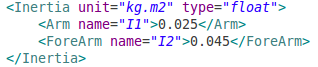
\includegraphics[scale=0.5]{XMLInertia.png}
\end{flushleft}

$<DampingTerm>$ is composed of $<bi>$ element where i is the number of the damping term. Each of these elements contain a float.
\begin{flushleft}
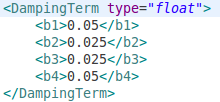
\includegraphics[scale=0.5]{XMLDamping.png}
\end{flushleft}

$<MomentMatrix>$ is composed of $<mi>$ elements where i is the number of the moment element. Each of these elements contain a float.
\begin{flushleft}
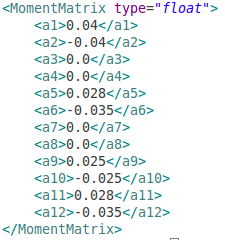
\includegraphics[scale=0.5]{XMLMoment.png}
\end{flushleft}

$<Bounds>$ is composed of one elements for each joint. The joint element is named with the joint name and contain a $<Lower>$ and a $<Upper>$ elements for the lower and upper bounds.
\begin{flushleft}
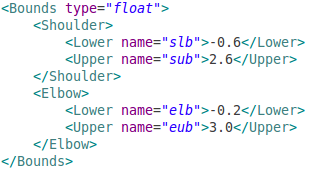
\includegraphics[scale=0.5]{XMLBounds.png}
\end{flushleft}
\subsubsection{Muscles setup}
The name of the structure setup file is "MusclesParamsDM.xml" where D is the number of degrees of freedom of the arm and M the number of muscles.
The root element is $<Muscle>$ and it is composed of two elements $<MaximumForce>$ and $<Knoise>$.
$<MaximumForce>$ contain a elements for each muscles. These elements contains the maximun force of the related muscle.
\begin{flushleft}
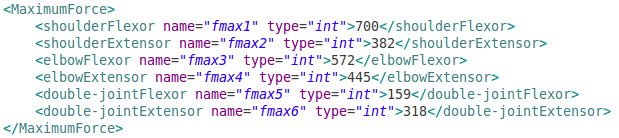
\includegraphics[scale=0.5]{XMLForce.png}
\end{flushleft}
The $<Knoise>$ element contain a float that is the noise parameter for the muscles activation.
\begin{flushleft}
\includegraphics[scale=0.5]{XMLKnoise.png}
\end{flushleft}
\subsection{Global setup}
\label{global}
The root of this setup file is $<setup>$. It is composed of 10 elements.
$<data>$ element contain data information : the size of the input, the size of the output, and if there is noise or not. The Arm module used is determined by the input or the output size (the size of the input is two x the number of joints and the size of the output is the number of muscles). Only the Arm with two joints and six muscle have been tested.
The next element is $<regression>$, it contain parameters of the regression module used. Its elements are the regression elements used (curently RBFN or NeuralNet), $<thetaFile>$ for the name of output parameters file and $<resultPath>$ for the directory where save the result. 
\subsubsection*{RBFN}
The $<RBFN>$ elements is composed of $<nbFeatures>$, $<lambda>$ and $<fromStruct>$.
$<nbFeatures>$ is the numbers of features, it is an integer.
$<lambda>$ is a float and $<fromStruct>$ is a string(yes or no) meaning if it use a structure from a previous RBFN or a new.
\subsubsection*{NeuralNet}
The $<NeuralNet>$ elements is composed of $<inputLayer$, $<hiddenLayers>$, $<outputLayers>$, $<bias>$, $<learningrate>$ and $<momentum>$.
$<hiddenLayers>$ are compose of zero or any number of $<hiddenLayer>$ we want. Each layer elements contains an element type, the different type are described in the Neural Network section. Furthermore $<hiddenLayer>$ have a $<size>$ element that contain the size of the layer. The size of the input and output layers are the input and output data size.
$<bias>$ is a string (yes or no) meaning if it use a bias or no. $<learningrate>$ and $<momentum>$ are float numbers.
\begin{flushleft}
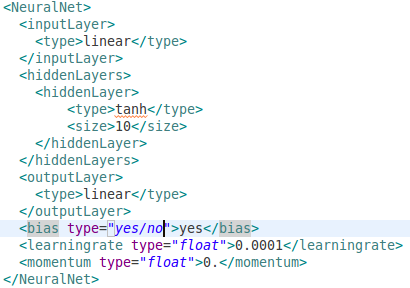
\includegraphics[scale=0.5]{XMLNeuralNet.png}
\end{flushleft}
The next element is $<costFunction>$, it contain the parameters of the cost function : gamma, rho and upsilon and the python class used.
\begin{flushleft}
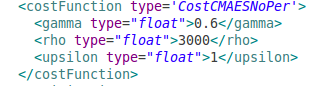
\includegraphics[scale=0.5]{XMLCost.png}
\end{flushleft}
Then we have the $<optimization>$ element that have an attribute type, for the type of the optimization done (CMAES or DDPG). For both types we have elements $<maxIteration>$, $<numberRepetition>$, $<resultPath>$.
Furthermore for CMAES type, we have two other elements $<sigma>$ and $<popsize>$.
\begin{flushleft}
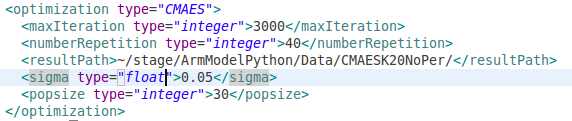
\includegraphics[scale=0.5]{XMLOpti.png}
\end{flushleft}
Then we have the target information (sizes and coordinate).
\begin{flushleft}
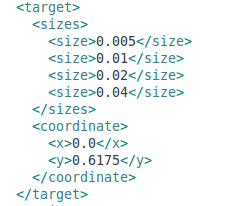
\includegraphics[scale=0.5]{XMLTarget.png}
\end{flushleft}
The trajectory information, <initialPosition> is the name of the file that contain the coordinate of the trajectory initial points.
\begin{flushleft}
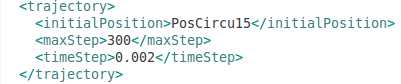
\includegraphics[scale=0.5]{XMLTraj.png}
\end{flushleft}
In the estimation element, we find the type of the estimation and the delay.  
\begin{flushleft}
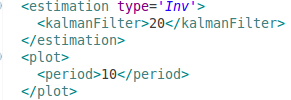
\includegraphics[scale=0.5]{XMLEstim.png}
\end{flushleft}

\section{Package Overview}
\subsection{ArmModel}
The package ArmModel contain all the file related to the arm model, Arm.py is a abstract class, the arm model need to inherit. Arm26.py and Arm38.py are the arm model already implemented. The *XML.py file parse the * setup file in ArmModel/Setup.
\subsection{Cost}
This package contains all different cost implemented. CostType is a dictionary of all cost.
\subsection{DDPG}
This package contains the DDPG algorithm.
\subsection{Experiment}
This package contains all different state estimator, there are referenced in StateEstimatorType. TrajMaker.py contains the tools to compute one trajectory, Experiments.py use TrajMaker to run all trajectories.
\subsection{Main}
In MainCMAES.py (rsp. MainDDPG.py) we found all the operation for the optimization with CMAES(rsp. DDPG).
\subsection{Optimizer}
This package contains the DDPG environments and the Bayesian Optimization. For more detail about the Bayesian optimization used see 
\url{https://github.com/fmfn/BayesianOptimization} 

\subsection{Plot}
This package contains the plot function.
\subsection{Regression}
This package contains the regressions class, all regression have to inherit from Regression.py.
DataSet.py is used to handle a data set, and RunRegression to handle a regression.
\subsection{Utils}
In this package, we find several tools, the like files and xml files readers, the chronometer and a distribution comparator.




\end{document}